\documentclass[12pt, titlepage, french]{report}
% Extra note : this preamble creates document that are meant to be used inside the multicols environment. See the documentation on internet for further information.

%% -----------------------------
%% Encoding packages
%% -----------------------------
\usepackage[utf8]{inputenc}
\usepackage[T1]{fontenc}
\usepackage{babel}
\usepackage{lmodern}
%
%%% -----------------------------
%%% Variable definition
%%% -----------------------------
%\def\auteur{Alec James van Rassel}
%\def\BackgroundColor{white}
%
%%% -----------------------------
%%% Margin and layout
%%% -----------------------------
%% Determine the margin for cheatsheet
\usepackage[hmargin=1cm, vmargin=1.7cm]{geometry}
\usepackage{multicol}

%% -----------------------------
%% URL and links
%% -----------------------------
\usepackage{hyperref}
\hypersetup{colorlinks = true, urlcolor = white, linkcolor = black}

%% -----------------------------
%% Document policy (uncomment only one)
%% -----------------------------
%	\usepackage{concrete}
%	\usepackage{mathpazo}
%	\usepackage{frcursive} %% permet d'écrire en lettres attachées
%	\usepackage{aeguill}
%	\usepackage{mathptmx}
%	\usepackage{fourier} 

%% -----------------------------
%% Math configuration
%% -----------------------------
\usepackage[fleqn]{amsmath}
\usepackage{amsthm,amssymb,latexsym,amsfonts}
\usepackage{empheq}
\usepackage{numprint}
\usepackage{dsfont} % Pour avoir le symbole du domaine Z

% Mathematics shortcuts

\newcommand{\reels}{\mathbb{R}}
\newcommand{\entiers}{\mathbb{Z}}
\newcommand{\naturels}{\mathbb{N}}
\newcommand{\eval}{\biggr \rvert}
\usepackage{cancel}
\newcommand{\derivee}[1]{\frac{\partial}{\partial #1}}
\newcommand{\prob}[1]{\Pr \left( #1 \right)}
\newcommand{\esp}[1]{\mathrm{E} \left[ #1 \right]} % espérance
\newcommand{\variance}[1]{\mathrm{Var} \left( #1   \right)}
\newcommand{\covar}[1]{\mathrm{Cov} \left( #1   \right)}
\newcommand{\laplace}{\mathcal{L}}
\newcommand{\deriv}[2][]{\frac{\partial^{#1}}{\partial #2^{#1}}}
\newcommand{\e}[1]{\mathrm{e}^{#1}}
\newcommand{\te}[1]{\text{exp}\left\{#1\right\}}
\DeclareMathSymbol{\shortminus}{\mathbin}{AMSa}{"39}

% To indicate equation number on a specific line in align environment
\newcommand\numberthis{\addtocounter{equation}{1}\tag{\theequation}}

%
% Actuarial notation packages
%
\usepackage{actuarialsymbol}
\usepackage{actuarialangle}

%
% Matrix notation for math symbols (\bm{•})
%
\usepackage{bm}
% Matrix notation variable (bold style)
\newcommand{\matr}[1]{\mathbf{#1}}


%% -----------------------------
%% tcolorbox configuration
%% -----------------------------
\usepackage[most]{tcolorbox}
\tcbuselibrary{xparse}
\tcbuselibrary{breakable}
%%	-----------------------------
%%
%%	Arguments
%%	+	breakable: allows box to be split over several pages
%%	+	segmentation style: To customize the \tcbline seperator
%%	
%%	-----------------------------
%%
%%
%% Coloured box "definition" for definitions
%%
%%
%% Coloured box "definition2" for definitions
%%
\DeclareTColorBox{definitionNOHFILL}{ o }				% #1 parameter
{
	colframe=blue!60!green,colback=blue!5!white, % color of the box
	pad at break* = 0mm, 						% to split the box
	title = {#1},
	before title = {\faBook \quad },
	breakable
}
%%
%% Coloured box "definition2" for definitions
%%
\DeclareTColorBox{definitionNOHFILLsub}{ o }				% #1 parameter
{
	colframe=blue!40!green,colback=blue!5!white, % color of the box
	pad at break* = 0mm, 						% to split the box
	title = {#1},
	before title = {\faNavicon \quad }, %faBars  faGetPocket
	breakable
}
\DeclareTColorBox{theorems}{ o}			% #1 parameter
{
	enhanced,
	title = #1,
	colback=bluebell, % color of the box
	colframe=blue(pigment),
	colbacktitle=blue!80!black,
	fonttitle = \bfseries,
	boxed title style={size=small,colframe=purple!50!black} ,
	attach boxed title to top center = {yshift=-3mm,yshifttext=-1mm},
	left=0pt,
  	right=0pt,
    box align=center,
    ams align*
%  	top=-10pt
}
\DeclareTColorBox{distributions}{ o }			% #1 parameter
{
	enhanced,
	title = #1,
	colback=ashgrey, % color of the box
%	colframe=blue(pigment),
%	colframe=lightgray,	
	colbacktitle=aurometalsaurus,
	fonttitle = \bfseries,
	boxed title style={size=small,colframe=arsenic} ,
	attach boxed title to top center = {yshift=-3mm,yshifttext=-1mm},
%	left=0pt,
%  	right=0pt,
%    box align=center,
%    ams align*
%  	top=-10pt
}
\DeclareTColorBox{astuces}{ o }			% #1 parameter
{
	enhanced,
	title = #1,
	colback=beaublue, % color of the box
%	colframe=blue(pigment),
	colframe=ballblue,	
	colbacktitle=aurometalsaurus,
	fonttitle = \bfseries,
	boxed title style={size=small,colframe=arsenic} ,
	attach boxed title to top center = {yshift=-3mm,yshifttext=-1mm},
%	left=0pt,
%  	right=0pt,
%    box align=center,
%    ams align*
%  	top=-10pt
}
\DeclareTColorBox{outcomes}{ o }			% #1 parameter
{
	enhanced,
	title = #1,
	colback=bluebell, % color of the box
%	colframe=blue(pigment),
%	colframe=asparagus,	
	colbacktitle=airforceblue,
	fonttitle = \bfseries,
	boxed title style={size=small,colframe=arsenic} ,
	attach boxed title to top center = {yshift=-3mm,yshifttext=-1mm},
%	left=0pt,
%  	right=0pt,
%    box align=center,
%    ams align*
%  	top=-10pt
}
\DeclareTColorBox{ASM_chapter}{ o }			% #1 parameter
{
	enhanced,
	title = #1,
	colback=darkseagreen, % color of the box
%	colframe=blue(pigment),
%	colframe=asparagus,	
	colbacktitle=britishracinggreen,
	fonttitle = \bfseries,
	boxed title style={size=small,colframe=arsenic} ,
	attach boxed title to top center = {yshift=-3mm,yshifttext=-1mm},
	segmentation style = {dashed, white},
	breakable
%	left=0pt,
%  	right=0pt,
%    box align=center,
%    ams align*
%  	top=-10pt
}
\DeclareTColorBox{YTB_vids}{ o }			% #1 parameter
{
	enhanced,
	title = #1,
	colback=red_rectangle, % color of the box
%	colframe=blue(pigment),
%	colframe=asparagus,	
	colbacktitle=lava,
	fonttitle = \bfseries,
	boxed title style={size=small,colframe=arsenic} ,
	attach boxed title to top center = {yshift=-3mm,yshifttext=-1mm},
	segmentation style = {dashed, white},
	breakable
%	left=0pt,
%  	right=0pt,
%    box align=center,
%    ams align*
%  	top=-10pt
}
%%
%% Coloured box "algo" for algorithms
%%
\newtcolorbox{algo}[ 1 ]
{
	colback = blue!5!white,
	colframe = blue!75!black,
	fonttitle = \bfseries,title=#1
}
%%
%% Coloured box "formula" for formulas
%%
\newtcolorbox{formula}[ 1 ]
{
	colback = beaublue,
	colframe = airforceblue,
	fonttitle = \bfseries,title=#1
}
%%
%% Coloured box "CHPT_SUMM" pour résumés des chapitres de l'ASM
%%
\newtcolorbox{CHPT_SUMM}[ 1 ]
{
	colback = green!5!white,
	colframe = darkseagreen,
	breakable,
	fonttitle = \bfseries,title=#1
}
%%
%% Coloured box "FORMULA_SUMM" pour résumés des formules de l'ASM
%%
\newtcolorbox{FORMULA_SUMM}[ 1 ]
{
	colback = babyblueeyes,
	colframe = airforceblue,
	breakable,
	fonttitle = \bfseries,title=#1
}
%%
%% Coloured box "YTB_SUMM" pour résumés des vidéos Youtube
%%
\newtcolorbox{YTB_SUMM}[ 1 ]
{
	colback = red!5!white,
	colframe = darkterracotta,
	breakable,
%	    frame hidden,
	fonttitle = \bfseries,title=#1
}
\newtcolorbox[auto counter, list inside = CHPT]{YTB_SUMM_AUTO_NUMB}[ 2 ][]
{
	colback = red!5!white,
	colframe = darkterracotta,
	breakable,
	enhanced,
	fonttitle = \bfseries,
	title = Video~\thetcbcounter: #2, 		
%	title = #2,
	nameref = #2,
	after upper = {\addcontentsline{toc}{subsubsection}{\thetcbcounter: #2}},
%	phantomlabel = {#2},
	#1
}
%%
%% Coloured box "rappel" pour rappel de formules
%%
\DeclareTColorBox{rappel_enhanced}{ o }
{
	enhanced,
	title = #1,
	colback=lightgray, % color of the box
%	colframe=blue(pigment),
%	colframe=arsenic,	
	colbacktitle=arsenic,
	fonttitle = \bfseries,
	breakable,
	boxed title style={size=small,colframe=arsenic} ,
	attach boxed title to top center = {yshift=-3mm,yshifttext=-1mm},
}
%%
%% Coloured box "FORMULA_SUMM" pour résumés des formules de l'ASM
%%
%% -----------------------------
%% Graphics and pictures
%% -----------------------------
\usepackage{graphicx}
\usepackage{pict2e}
\usepackage{tikz}
%%
%%	Creates circle 
%%	Arguments:
%%	+	size
%%	+	colour
%%	
%%	Example:
%%	+	\tikzcircle[green, fill=blue]{1.5pt}
%%	+	\tikzcircle{2pt}
%%
\newcommand{\tikzcircle}[2][red,fill=red]{\tikz[baseline=-0.5ex]\draw[#1,radius=#2] (0,0) circle ;}


%% -----------------------------
%% insert pdf pages into document
%% -----------------------------
\usepackage{pdfpages}

%% -----------------------------
%% Color configuration
%% -----------------------------
\usepackage{color, soulutf8, colortbl}

%
%	Colour definitions
%
\definecolor{ceruleanblue}{rgb}{0.16, 0.32, 0.75}
\definecolor{darkterracotta}{rgb}{0.8, 0.31, 0.36}   % red pastel ish
\definecolor{lava}{rgb}{0.81, 0.06, 0.13}
\definecolor{wildwatermelon}{rgb}{0.99, 0.42, 0.52}  % red ish
\definecolor{bostonuniversityred}{rgb}{0.8, 0.0, 0.0} % rich red
\definecolor{asparagus}{rgb}{0.53, 0.66, 0.42}		% sorta militarygreen but pastel
\definecolor{darkseagreen}{rgb}{0.56, 0.74, 0.56}    % pastel light green
\definecolor{britishracinggreen}{rgb}{0.0, 0.26, 0.15} %dark green
\definecolor{airforceblue}{rgb}{0.36, 0.54, 0.66}	% nice teal blue pastel
\definecolor{babyblueeyes}{rgb}{0.63, 0.79, 0.95}	% pastel blue-ish
\definecolor{applegreen}{rgb}{0.55, 0.71, 0.0}		% green with some aqua
\definecolor{indigo(web)}{rgb}{0.29, 0.0, 0.51}
\definecolor{cobalt}{rgb}{0.0, 0.28, 0.67}
\definecolor{azure(colorwheel)}{rgb}{0.0, 0.5, 1.0}
\definecolor{darkpastelpurple}{rgb}{0.59, 0.44, 0.84}
\definecolor{darkgreen}{rgb}{0.0, 0.2, 0.13}			
\definecolor{burntorange}{rgb}{0.8, 0.33, 0.0}		
\definecolor{burntsienna}{rgb}{0.91, 0.45, 0.32}		
\definecolor{ao(english)}{rgb}{0.0, 0.5, 0.0}		% ACT-2003
\definecolor{amber(sae/ece)}{rgb}{1.0, 0.49, 0.0} 	% ACT-2004
\definecolor{green_rectangle}{RGB}{131, 176, 84}		% ACT-2004
\definecolor{red_rectangle}{RGB}{241,112,113}		% ACT-2004
\definecolor{blue_rectangle}{RGB}{83, 84, 244}		% ACT-2004
\definecolor{blue(pigment)}{rgb}{0.2, 0.2, 0.6}
\definecolor{bluebell}{rgb}{0.64, 0.64, 0.82}
\definecolor{amethyst}{rgb}{0.6, 0.4, 0.8}
\definecolor{amethyst-light}{rgb}{0.6, 0.4, 0.8}
\definecolor{aurometalsaurus}{rgb}{0.43, 0.5, 0.5}
\definecolor{arsenic}{rgb}{0.23, 0.27, 0.29}			%	dark black-grey ish pastel
\definecolor{ashgrey}{rgb}{0.7, 0.75, 0.71}
\definecolor{beaublue}{rgb}{0.74, 0.83, 0.9}
\definecolor{ballblue}{rgb}{0.13, 0.67, 0.8}
\definecolor{lightgray}{rgb}{0.83, 0.83, 0.83}
\definecolor{antiquefuchsia}{rgb}{0.57, 0.36, 0.51}
%
% Useful shortcuts for coloured text
%
\newcommand{\orange}{\textcolor{orange}}
\newcommand{\red}{\textcolor{red}}
\newcommand{\cyan}{\textcolor{cyan}}
\newcommand{\blue}{\textcolor{blue}}
\newcommand{\green}{\textcolor{green}}
\newcommand{\purple}{\textcolor{magenta}}
\newcommand{\yellow}{\textcolor{yellow}}

%% -----------------------------
%% Enumerate environment configuration
%% -----------------------------
%
% Custum enumerate & itemize Package
%
\usepackage{enumitem}
%
% French Setup for itemize function
%
\frenchbsetup{StandardItemLabels=true}
%
% Change default label for itemize
%
\renewcommand{\labelitemi}{\faAngleRight}


%% -----------------------------
%% Tabular column type configuration
%% -----------------------------
\newcolumntype{C}{>{$}c<{$}} % math-mode version of "l" column type
\newcolumntype{L}{>{$}l<{$}} % math-mode version of "l" column type
\newcolumntype{R}{>{$}r<{$}} % math-mode version of "l" column type
\newcolumntype{f}{>{\columncolor{green!20!white}}p{1cm}}
\newcolumntype{g}{>{\columncolor{green!40!white}}m{1.2cm}}
\newcolumntype{a}{>{\columncolor{red!20!white}$}p{2cm}<{$}}	% ACT-2005
% configuration to force a line break within a single cell
\usepackage{makecell}


%% -----------------------------
%% Fontawesome for special symbols
%% -----------------------------
\usepackage{fontawesome}

%
%%% -----------------------------
%%% Footer/Header Customization
%%% -----------------------------
\usepackage{lastpage}
\usepackage{fancyhdr}
\pagestyle{fancy}
%%
%% Page background color
%%
\pagecolor{white}

%% -----------------------------
%% Section Font customization
%% -----------------------------
\usepackage{sectsty}
%\sectionfont{\color{\SectionColor}}
%\subsectionfont{\color{\SubSectionColor}}



\usepackage{ctable}
%% END OF PREAMBLE
% ---------------------------------------------
% ---------------------------------------------
%% -----------------------------
%% Section Font customization
%% -----------------------------
%\title{
%	Study Guide	\\
%	\large Exam YYY: Name-of-Exam\\
%	Society of Actuaries (SOA)
%%	Casualty Actuarial Society (CAS)
%	}
%\vspace{-8ex}
%\date{}
%\author{Alec James van Rassel}

\begin{document}

%\maketitle

\tableofcontents

\clearpage

\part*{Statistics}

\section*{Missing Data}

\begin{YTB_vids}[Vidéos YouTube]
\begin{itemize}
	\item	\nameref{rvm-MCAR-etal}
	\item	\nameref{rvm-MCAR-etal-deal}
	\item	\nameref{rvm-MCAR-etal-mult}
	\item	
\end{itemize}
\end{YTB_vids}

\subsection*{Notes sur les vidéos YouTube}

\begin{YTB_SUMM_AUTO_NUMB}[label = {rvm-MCAR-etal}]{\href{https://www.youtube.com/watch?v=XnnA9z7lv4Q}{ritvikmath: Missing Data Mechanisms
}}
\begin{itemize}[leftmargin = *]
	\item	MCAR
		\begin{itemize}
		\item	Librarians forget to enter the data completely randomly;
		\end{itemize}
	\item	MAR
		\begin{itemize}
		\item	Women are 90\% likely to respond to a survey on the number of overdue books while men are 70\% likely to respond;
		\end{itemize}
	\item	MNAR: \textbf{The missingness of a certain value depends on the true value itself}
		\begin{itemize}
		\item	For example:
			\begin{itemize}
			\item	If I have 0 books overdue, I'm 90\% likely to respond to a question asking how many overdue books I have;
			\item	If I have 1 books overdue, I'm 80\% likely to respond to a question asking how many overdue books I have;
			\item	If I have 2 books overdue, I'm 70\% likely to respond to a question asking how many overdue books I have;
			\item	\dots
			\end{itemize}
		\item	So, the more books I have that are overdue, the less likely I am to respond to a question asking how many books I have that are overdue because I may be embarassed or feel shame;
		\item	Therefore MNAR is kind of a \textbf{chicken and egg} scenario;
			\begin{itemize}
				\item	If try to figure if a column is MNAR, need to figure out if those missing values are based on the actual values;
				\item	But, I \textit{don't know} the \textbf{actual} values of that column because they're missing in the first place!
				\item	So it's really hard to figure out if something is MNAR;
			\end{itemize}
		\end{itemize}
	\begin{itemize}
	\item	In comparision, MCAR and MAR are easier to figure out if something is one or the other;
	\item	Can slice a dataset by values of a column
		\begin{itemize}
		\item	For example, by sex or by age group, \dots;
		\item	If missing value rate is about the same for all different slices then likely to be Missing Completely At Random;
		\item	If however it's different for each slice, then it's likely MAR;
		\end{itemize}
	\end{itemize}
\end{itemize}
\end{YTB_SUMM_AUTO_NUMB}

\begin{YTB_SUMM_AUTO_NUMB}[label = {rvm-MCAR-etal-deal}]{\href{https://www.youtube.com/watch?v=qIXHLZJJ42U}{ritvikmath: Dealing With Missing Data Part I}}
\begin{itemize}[leftmargin = *]
	\item	Row deletion;	
		\begin{itemize}
		\item	Most common and easiest;
		\item	Omit any row in dataset with a missing value---pretend it does not exist;
		\item	Seems too good to be true because it usually is;
		\item	Can only do this if the data is Missing Completely At Random---biased otherwise;
		\item[]	Makes sense if you reason that any other way you'd obviously be creating a bias in your data;
		\item[]	Each column would have missing values completely at random and without respect to, for example, the gender and the estimations would be \textit{unbiased};
		\item	Thus, have to be very careful it's really what we want to do because likely cause bias if there's any sort of relationship between the missing variables and other columns;
		\end{itemize}
	\begin{center}
	\begin{tabular}{| >{\columncolor{beaublue}}c | >{\columncolor{beaublue}}c |}
	\hline\rowcolor{airforceblue} 
		\textcolor{white}{\textbf{Pros}}	&	\textcolor{white}{\textbf{Cons}}	\\
simple	&	\textbf{biased}	\\\hline
	\end{tabular}
	\end{center}
	\item	Mean/Median imputation;
		\begin{itemize}
		\item	A little more \og clever \fg{};
		\item	\textbf{Seems} intuitive and is pretty simple;
		\item	Mean
			\begin{itemize}[leftmargin = *]
			\item	Fill in, for example, 1.8 as the average of a few discrete values;
			\item	BUT, will \textbf{artifically} \textit{reduce variability} of the data;
			\item	\textit{Seem} like several values have the exact same value;
			\end{itemize}
		\item	Median is the same idea but will overepresent one fixed value;
		\end{itemize}
	\begin{center}
	\begin{tabular}{| >{\columncolor{beaublue}}c | >{\columncolor{beaublue}}c |}
	\hline\rowcolor{airforceblue} 
		\textcolor{white}{\textbf{Pros}}	&	\textcolor{white}{\textbf{Cons}}	\\
simple	&	\textbf{lower variability}	\\\hline
	\end{tabular}
	\end{center}
	\item	Hot Deck methods;
		\begin{itemize}
		\item	Most clever so far;
		\item	Any family of methods where:
			\begin{itemize}[leftmargin = *]
			\item	Compute a missing value based on the value of examples that are \textit{similar} to it;
			\end{itemize}
		\item	For example
			\begin{itemize}
			\item	Fill in the missing value of a female by the average of only other females;
			\end{itemize}
		\item	Better because imputing more information (whether someone is female or male);
			\begin{itemize}
			\item	Imagine if there's a bunch of columns (income, family members, where they live, etc.);
			\item	Then, we can input missing values based on a few people that are really similar to the missing person;
			\item	Logical as we would expect that person's missing value to be similar to other similar people's;
			\end{itemize}
		\item	\textbf{May not be true}, but it's a very \textit{\textbf{educated} guess};
		\end{itemize}
	\begin{center}
	\begin{tabular}{| >{\columncolor{beaublue}}c | >{\columncolor{beaublue}}c |}
	\hline\rowcolor{airforceblue} 
		\textcolor{white}{\textbf{Pros}}	&	\textcolor{white}{\textbf{Cons}}	\\
more educated	&	more (computationnaly) expensive	\\\hline
	\end{tabular}
	\end{center}
\end{itemize}
\end{YTB_SUMM_AUTO_NUMB}

\begin{YTB_SUMM_AUTO_NUMB}[label = {rvm-MCAR-etal-mult}]{\href{https://www.youtube.com/watch?v=LMsULWGtP2c}{ritvikmath: Dealing With Missing Data - Multiple Imputation}}
\begin{itemize}[leftmargin = *]
	\item	\textit{single} imputation implique qu'on se ramasse avec une seule valeur (peu importe ce que c'est);
		\begin{itemize}
		\item	Régression, moyenne, médiane, etc. sont tous une seule valeur.
		\end{itemize}
	\item	\textit{multiple} imputation even more clever than hot-deck methods;
	\item	For example, regression of library fees in function of kilometer distance from the library
		\begin{itemize}[leftmargin = *]
		\item	Sample 50 data points from thousands, and estimate fees for a given distance;
		\item	Repeat with different samples;
		\item[]	Generally the more repetitions, the less biased the estimations but 5 is a good rule of thumb;
		\item	Treat each predicted value as a complete observation;
		\item	Then with this "complete" data set, we do what we want;
		\item	Take some kind of aggregate of all the values we wanted from each of 5-ish set;
		\item	Analyze how far from each other the aggregated values are;
		\item[]	If a lot of variability, bad;
		\item[]	If few variability, good-ish because means aggregated values are closer.	
		\end{itemize}
		\begin{center}
			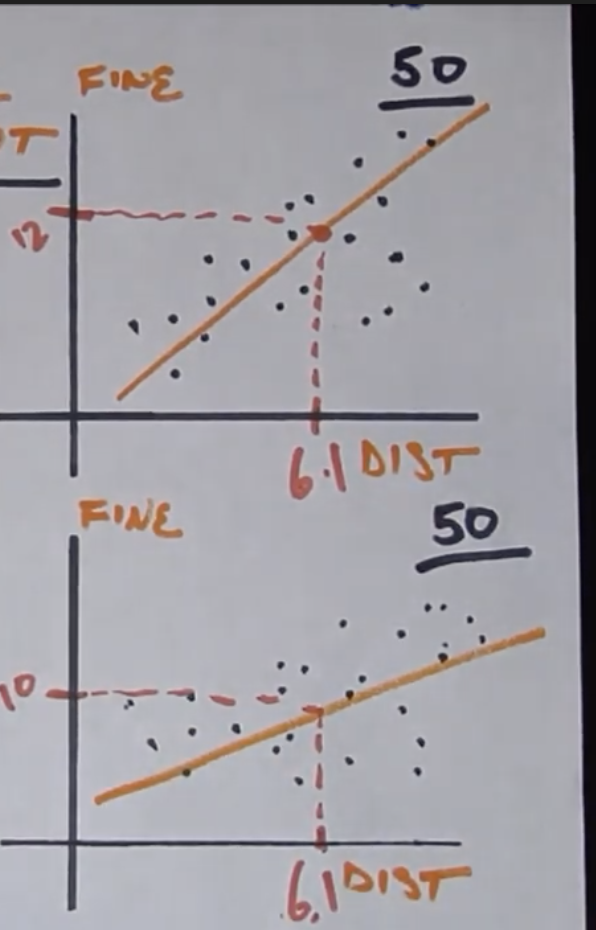
\includegraphics[scale=0.3]{src/ritvikmath-multiple-imputation.png}
		\end{center}
	\item	Cons: complicated.
\end{itemize}
\end{YTB_SUMM_AUTO_NUMB}

\newpage

\end{document}
